\documentclass{article}
\usepackage{graphicx} % Requerido para insertar imágenes
\usepackage{amsmath}  % Para ecuaciones
\usepackage{amssymb}  % Para símbolos
\usepackage{hyperref} % Para enlaces (opcional)
\usepackage{setspace}
\usepackage{fancyhdr} % Para encabezados/pies de página
\usepackage{titlesec} % Para formato de títulos
\usepackage{geometry} % Para márgenes
\usepackage{tikz}
\usetikzlibrary{arrows.meta, positioning, calc}

\geometry{margin=2.5cm}

% --- Configuración de encabezados y pies de página ---
\pagestyle{fancy}
\fancyhf{}
\fancyfoot[C]{\thepage}
\fancyhead[L]{Deber 2 - Seguridad Informática}
\fancyhead[R]{Xavier Sebastián Tandazo Cobo}

% --- Título ---
\title{\vspace{-2cm}\textbf{Deber 2 - Seguridad Informática}\\[4pt]
Universidad San Francisco de Quito\\[2pt]}
\author{Xavier Sebastián Tandazo Cobo}
\date{13 de noviembre de 2025}

\begin{document}

\maketitle
\thispagestyle{empty} % Quita encabezado/pie de la primera página
\newpage % Inicia el contenido en una nueva página

\section*{Pregunta 1: Firma Digital Estándar y Análisis de Mecanismos Alternativos}

\subsection{Protocolo Estándar de Firma Digital}

Para poder ilustrar el funcionamiento del protocolo estándar de firma digital de una manera entendible, consideremos el siguiente ejemplo:

\begin{quote}
    Alice desea enviar a Bob el mensaje: \textit{``Transferir \$100 a la cuenta de Mark''}. 
    Ella quiere garantizar que Bob pueda verificar que el mensaje proviene realmente de ella y que no ha sido modificado durante la transmisión.
\end{quote}

Como se explica en el enunciado del deber, este proceso se desarrolla en cuatro etapas principales:

% --- Gráfico del protocolo estándar ---
\begin{figure}[h!]
\centering
\begin{tikzpicture}[
    node distance=1.3cm and 2cm,
    >=Latex,
    process/.style={rectangle, draw, rounded corners, align=center, minimum width=3cm, minimum height=1cm},
    actor/.style={ellipse, draw, align=center, minimum width=2cm, minimum height=1cm, fill=gray!10},
    data/.style={rectangle, draw, align=center, minimum width=3.3cm, minimum height=0.8cm, fill=blue!5},
    arrow/.style={->, thick}
]

% --- Nodos principales ---
\node[actor] (alice) {Alice};
\node[actor, right=8cm of alice] (bob) {Bob};

% --- Etapas de Alice ---
\node[process, below=of alice] (hash) {1. Hash del mensaje \\ $H(M) = \text{SHA256}(M)$};
\node[data, below=0.3cm of hash] (hashval) {$H(M)$};
\node[process, below=of hashval] (sign) {2. Firma con clave privada \\ $Sig = E_{SK_{Alice}}(H(M))$};
\node[data, below=0.3cm of sign] (pair) {Par $(M, Sig)$};
\node[process, below=of pair] (send) {3. Envío a Bob};

% --- Flecha hacia Bob ---
\draw[arrow] (send.east) -- node[above, sloped]{Mensaje y Firma $(M, Sig)$} (bob.west);

% --- Etapas de Bob ---
\node[process, below=of bob] (verify1) {4a. Hash del mensaje recibido \\ $H(M') = \text{SHA256}(M')$};
\node[process, below=of verify1] (verify2) {4b. Descifra firma con clave pública \\ $H(M) = D_{PK_{Alice}}(Sig)$};
\node[process, below=of verify2] (compare) {Compara $H(M')$ y $H(M)$};
\node[data, below=0.3cm of compare] (result) {Si son iguales $\Rightarrow$ \\ 
Autenticidad ✓ \\ 
Integridad ✓ \\ 
No repudio ✓};

% --- Flechas de flujo en Alice ---
\draw[arrow] (alice.south) -- (hash);
\draw[arrow] (hash) -- (hashval);
\draw[arrow] (hashval) -- (sign);
\draw[arrow] (sign) -- (pair);
\draw[arrow] (pair) -- (send);

% --- Flechas de flujo en Bob ---
\draw[arrow] (bob.south) -- (verify1);
\draw[arrow] (verify1) -- (verify2);
\draw[arrow] (verify2) -- (compare);
\draw[arrow] (compare) -- (result);

% --- Título ---
\node[above=0.5cm of alice, align=center, font=\bfseries] (title)
{Protocolo Estándar de Firma Digital};

\end{tikzpicture}
\caption{Flujo del protocolo estándar de firma digital entre Alice y Bob.}
\end{figure}
% --- Fin del gráfico ---

\subsubsection*{1. Digest Computation}
Alice aplica una función hash criptográfica segura (diremos que la SHA-256) sobre el mensaje \( M \):
\[
H(M) = \text{SHA256}(\text{``Transferir \$100 a la cuenta Mark''})
\]
El resultado es un valor de longitud fija, por ejemplo:
\[
H(M) = \texttt{"hash-unico"}
\]
Un hash representa de forma única el contenido de un mensaje y cualquier cambio, por más mínimo, produciría un hash completamente diferente.

\subsubsection*{2. Signing}
Alice cifra su hash con su \textbf{clave privada} \( SK_{Alice} \):
\[
Sig = E_{SK_{Alice}}(H(M))
\]
Este valor cifrado (\( Sig \)) constituye la \textbf{firma digital}, pero solo Alice, al poseer su clave privada, puede generar este valor específico.

\subsubsection*{3. Transmission}
Alice envía a Bob el par \((M, Sig)\), es decir, el mensaje y la firma:
\[
(\text{``Transferir \$100 a la cuenta 1234''},\ Sig)
\]
El mensaje no necesita ser cifrado, ya que la firma digital garantiza autenticación e integridad, no confidencialidad.

\subsubsection*{4. Verification}
Bob realiza dos operaciones:
\begin{enumerate}
    \item Calcula el hash del mensaje recibido:
    \[
    H(M') = \text{SHA256}(\text{``Transferir \$100 a la cuenta 1234''})
    \]
    \item Descifra la firma usando la \textbf{clave pública} de Alice:
    \[
    H(M) = D_{PK_{Alice}}(Sig)
    \]
    Si \( H(M') = H(M) \), Bob puede concluir que:
    \begin{itemize}
        \item El mensaje proviene de Alice.
        \item No fue modificado.
        \item Alice no puede negar haberlo firmado.
    \end{itemize}
\end{enumerate}



\subsection{Análisis de Mecanismos Alternativos}

Siguiendo el objetivo del enunciado, se analizan dos esquemas alternativos que no cumplen con las propiedades criptográficas requeridas.

\subsubsection*{Mecanismo 1: Uso de criptografía simétrica}

\begin{quote}
En este esquema, se propone utilizar un sistema de clave simétrica en lugar de un esquema basado en criptografía de clave pública. 
El firmante y el receptor comparten una clave secreta común, usada tanto para generar como para verificar la ``firma''.
\end{quote}

A primera vista, este mecanismo puede parecer funcional, pero no cumple con las propiedades esenciales de una firma digital.  
La autenticación simétrica depende de confianza mutua, mientras que la firma digital extiende esa confianza a terceros, garantizando prueba verificable del origen del mensaje.  
De acuerdo con los principios descritos en \textit{Cryptography and Network Security}, este método puede autenticar, pero no ofrecer \textbf{no repudio} ni verificación independiente.

\paragraph{Problemas y propiedades violadas:}
\begin{itemize}
    \item \textbf{Pérdida del no repudio:} Ambos conocen la misma clave, por lo que cualquiera podría haber generado la firma.  
    \item \textbf{Dependencia del firmante en la verificación:} El receptor necesita que el emisor valide la firma, rompiendo la independencia.  
    \item \textbf{Riesgo de manipulación:} El receptor podría alterar el mensaje y solicitar una verificación, obteniendo firmas sobre contenido modificado.
\end{itemize}

\paragraph{Ejemplo:}
Si Alice y Bob comparten una clave $K_{AB}$, Alice ``firma'' el mensaje cifrando su hash:
\[
S = E_{K_{AB}}(H(M))
\]
Bob no puede verificarla sin reenviarla a Alice, eliminando la verificación independiente.  
Por tanto, este esquema \textbf{no cumple autenticación independiente ni no repudio}.

\subsubsection*{Mecanismo 2: Cifrado completo del mensaje con la clave privada}

\begin{quote}
En este mecanismo, el firmante cifra el mensaje completo $M$ con su clave privada, y el receptor lo descifra con la clave pública para obtener el mensaje y su autenticidad.
\end{quote}

Aun cuando parece ofrecer autenticidad, este esquema confunde cifrado con firma digital.  
Cifrar con la clave privada no protege la confidencialidad (ya que todos poseen la clave pública) y además es ineficiente.  
Según los principios del libro de Stallings, la firma debe aplicarse sobre un \textit{hash} del mensaje, no sobre el mensaje completo.

\paragraph{Problemas y propiedades violadas:}
\begin{itemize}
    \item \textbf{Ineficiencia:} Cifrar mensajes grandes con algoritmos asimétricos es costoso.  
    \item \textbf{Pérdida de confidencialidad:} Cualquier persona con la clave pública puede descifrar el contenido.
\end{itemize}

\paragraph{Ejemplo:}
Alice cifra el mensaje:
\[
C = E_{K_{priv}}(M)
\]
Bob lo descifra con la clave pública:
\[
M = D_{K_{pub}}(C)
\]
El resultado es el mensaje original, pero cualquiera puede hacer lo mismo.  
Por tanto, este esquema sacrifica \textbf{eficiencia, confidencialidad y correcta semántica} de firma digital.

\subsection{Conclusión}
Ambos mecanismos fallan en reproducir las propiedades esenciales de las firmas digitales:  
el primero elimina el no repudio y la verificación independiente;  
el segundo confunde el cifrado con la firma digital, comprometiendo la eficiencia y confidencialidad.  
Solo el protocolo estándar basado en hash y firma asimétrica garantiza autenticidad, integridad y verificabilidad pública.

\newpage

\section*{Pregunta 2: Vulnerabilidad ante Vectores de Ataque}
Para esta pregunta, se plantea el siguiente escenario: 

\begin{quote}

Oscar actúa como un adversario que intenta comprometer la integridad y autenticidad de las comunicaciones entre Alice y Bob. 

\end{quote}

A continuación se analiza el funcionamiento, los posibles ataques, las vulnerabilidades explotadas y las soluciones criptográficas aplicables en cada caso.

\subsection{Escenario 1: Modificación del mensaje en tránsito}

\begin{quote}
Alice envía a Bob el mensaje:
\[
M = \text{``Transferir \$1000 a Mark''}
\]
junto con su correspondiente firma digital:
\[
auth(M)
\]
Oscar intercepta la transmisión y modifica el contenido del mensaje, cambiando el destinatario a:
\[
M' = \text{``Transferir \$1000 a Oscar''}
\]
\end{quote}

\subsubsection*{Análisis del ataque}

Oscar está ejecutando un \textbf{message tampering} (un ataque de manipulación de mensaje).  
Aunque no posee la clave privada de Alice, intenta modificar el mensaje durante la transmisión, esperando que Bob no detecte el cambio.

Pero al recibir el mensaje modificado, Bob calculará el valor hash del nuevo mensaje \( H(M') \) y lo comparará con el valor descifrado de la firma \( D_{PK_{Alice}}(auth(M)) \), que corresponde a \( H(M) \).  

Y entonces, como \( H(M) \neq H(M') \), se espera que la verificación de la firma falle inmediatamente.

\begin{center}
\begin{figure}[h!]
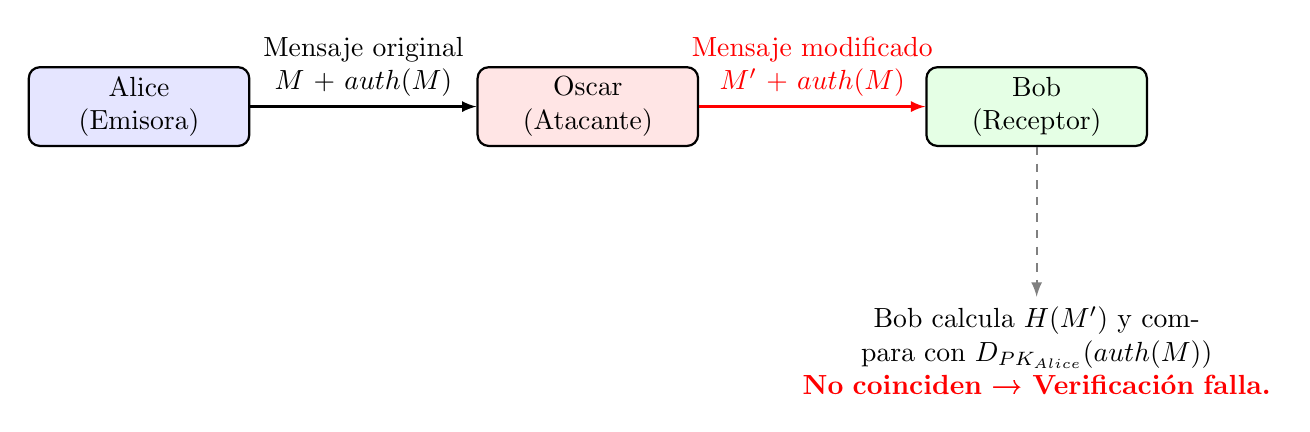
\begin{tikzpicture}[node distance=2.7cm,>=latex,thick]
    % Nodos principales
    \node (alice) [draw, rounded corners, fill=blue!10, align=center, minimum width=2.8cm, minimum height=1cm] {Alice\\(Emisora)};
    \node (oscar) [right of=alice, xshift=3cm, draw, rounded corners, fill=red!10, align=center, minimum width=2.8cm, minimum height=1cm] {Oscar\\(Atacante)};
    \node (bob) [right of=oscar, xshift=3cm, draw, rounded corners, fill=green!10, align=center, minimum width=2.8cm, minimum height=1cm] {Bob\\(Receptor)};

    % Flechas y etiquetas
    \draw[->, thick] (alice) -- node[above, text width=4cm, align=center] {Mensaje original \\ $M$ + $auth(M)$} (oscar);
    \draw[->, thick, red] (oscar) -- node[above, text width=4cm, align=center] {Mensaje modificado \\ $M'$ + $auth(M)$} (bob);

    % Flecha de verificación
    \node[below of=bob, yshift=-0.4cm, text width=6cm, align=center] (verify) {
        Bob calcula $H(M')$ y compara con $D_{PK_{Alice}}(auth(M))$\\
        \textbf{\textcolor{red}{No coinciden → Verificación falla.}}
    };

    % Flecha decorativa hacia abajo
    \draw[->, dashed, gray] (bob.south) -- (verify.north);
\end{tikzpicture}
\caption{Ilustración sobre como Bob se daría cuenta que el mensaje ha sido alterado.}
\end{figure}
\end{center}


\subsubsection*{Vulnerabilidad explotada}

En este escenario, Oscar intenta explotar la \textbf{ausencia de verificación de integridad}.  
Si, por ejemplo, Bob no validara la firma digital o el protocolo careciera de una función hash segura, el ataque sería un éxito.

\subsubsection*{Solución criptográfica}

La protección ante este tipo de ataque está garantizada por las propiedades inherentes a una \textbf{firma digital estándar}, que incluyen:
\begin{itemize}
    \item \textbf{Integridad:} cualquier modificación del mensaje cambia el hash.
    \item \textbf{Autenticidad:} solo Alice puede generar una firma válida.
\end{itemize}

\begin{center}
\textit{Resultado: Bob detectará la alteración, ya que la firma digital no coincidirá con el mensaje modificado.}
\end{center}

\subsection{Escenario 2: Ataque de repetición}

\begin{quote}
Oscar observa una transacción legítima enviada por Alice:
\[
M = \text{``Transferir \$1000 a Mark''}, \quad auth(M)
\]
y decide interceptarla y retransmitirla múltiples veces (por ejemplo, 100 veces) hacia Bob.
\end{quote}

\subsubsection*{Análisis del ataque}

Para este caso, Oscar no altera el contenido del mensaje ni la firma digital, sino que realiza un \textbf{replay attack}.  
El objetivo es engañar a Bob para que procese varias veces la misma instrucción de transferencia, generando así efectos económicos o lógicos repetidos.

Aunque la firma digital garantiza autenticidad e integridad, nunca se menciona protección contra la \textbf{reutilización de mensajes válidos}.  

Por lo que Bob, al recibir el mensaje idéntico con una firma válida, no tendría manera de distinguir si se trata de una retransmisión fraudulenta o de una comunicación legítima repetida.

\subsubsection*{Vulnerabilidad explotada}

Oscar se aprovecha de la \textbf{falta de mecanismos de frescura temporal o unicidad} en el protocolo, pues la firma digital por sí sola no incorpora información sobre cuándo o cuántas veces debe ser válida una transacción.

\subsubsection*{Soluciones criptográficas}

\begin{itemize}
    \item \textbf{Uso de números de identificadores únicos:} Cada mensaje debería incluir un valor único o incremental que el receptor verifique para evitar repeticiones.
    \item \textbf{Incorporación de marcas de tiempo:} Los mensajes se consideran válidos solo dentro de un intervalo temporal permitido.
\end{itemize}

Combinando estos mecanismos con firmas digitales, el sistema podría aspirar a garantizar no solo integridad y autenticación, sino también \textbf{protección frente a la reutilización maliciosa de mensajes}.

\begin{center}
\textit{Resultado: Bob no detectará la repetición si no hay control de unicidad. Se requiere incluir nonces o timestamps en el protocolo para evitar este tipo de ataque.}
\end{center}

\vspace{0.5cm}

\newpage
\section*{Pregunta 3: Investigación — TLS 1.3 (Transport Layer Security)}

\subsection{Evolución y Arquitectura del Protocolo TLS}

El protocolo \textbf{TLS (Transport Layer Security)} es la evolución del antiguo \textbf{SSL (Secure Socket Layer)} desarrollado originalmente por Netscape.  

Su función principal es proporcionar \textbf{confidencialidad, integridad y autenticación} entre dos aplicaciones que se comunican a través de la red; en términos de redes, se ubica entre la capa de transporte (TCP) y la capa de aplicación.

De acuerdo con material académico de seguridad informática, el SSL/TLS provee:
\begin{itemize}
    \item \textbf{Confidencialidad}, mediante cifrado simétrico.
    \item \textbf{Integridad}, a través de códigos de autenticación de mensaje (MAC o AEAD).
    \item \textbf{Autenticación}, gracias al uso de certificados digitales y firmas asimétricas.
\end{itemize}

En un inicio, SSL ofrecía estos servicios a través de un conjunto de subprotocolos jerárquicos, como \textit{Handshake, Change Cipher Spec,} y \textit{Alert}. TLS heredó esta estructura, pero la mejoró progresivamente en eficiencia y seguridad.

La versión \textbf{1.3 de TLS} representa una evolución significativa respecto a TLS 1.2:
\begin{itemize}
    \item Reduce el número de rondas en el \textit{Handshake}, logrando un establecimiento más rápido (1-RTT o incluso 0-RTT).
    \item Elimina algoritmos inseguros como RC4, MD5 y SHA-1.
    \item Introduce \textbf{Forward Secrecy}, asegurando que la exposición de una clave privada no comprometa sesiones pasadas.
    \item Simplifica la negociación de parámetros criptográficos, reduciendo la superficie de ataque.
\end{itemize}

TLS, al operar sobre TCP, se convierte en la base de servicios seguros como \textbf{HTTPS (HTTP over TLS)}, y también de otros protocolos como \textbf{SMTP}, \textbf{IMAP} y \textbf{FTPS}.

\vspace{0.4cm}
\begin{figure}[h!]
\centering
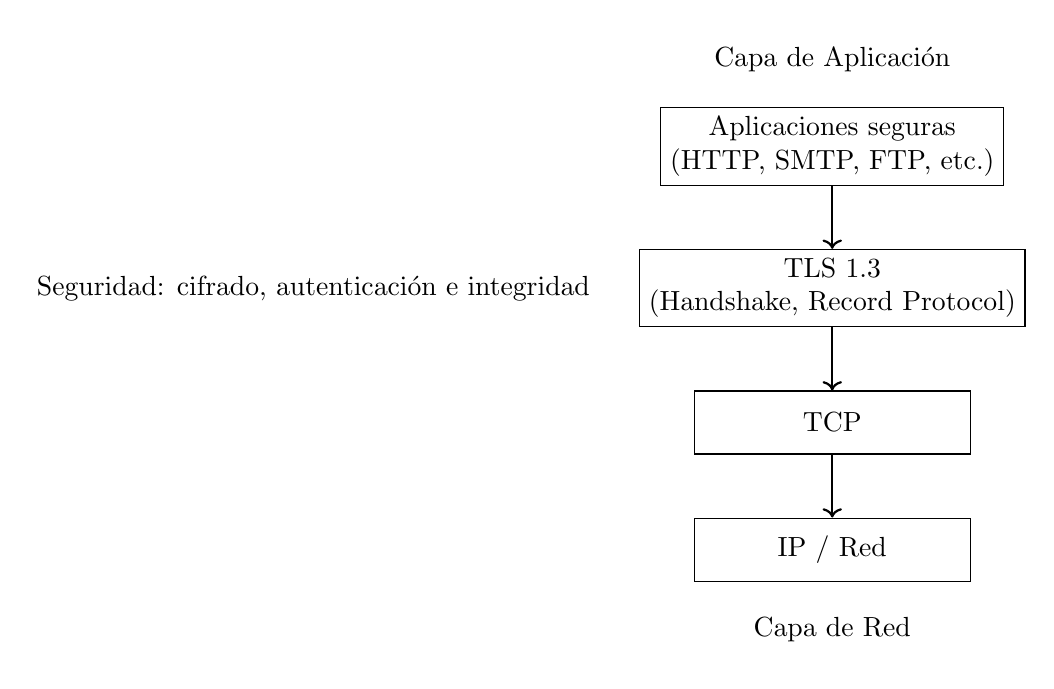
\begin{tikzpicture}[node distance=0.8cm, every node/.style={rectangle, draw, minimum width=3.5cm, minimum height=0.8cm, align=center}]

% Capas de la arquitectura
\node (apps) {Aplicaciones seguras \\ (HTTP, SMTP, FTP, etc.)};
\node (tls) [below=of apps] {TLS 1.3 \\ (Handshake, Record Protocol)};
\node (tcp) [below=of tls] {TCP};
\node (ip) [below=of tcp] {IP / Red};

% Flechas de comunicación
\draw[->, thick] (apps.south) -- (tls.north);
\draw[->, thick] (tls.south) -- (tcp.north);
\draw[->, thick] (tcp.south) -- (ip.north);

% Etiquetas de servicios
\node[draw=none, above=0.2cm of apps] {Capa de Aplicación};
\node[draw=none, left=0.5cm of tls] {Seguridad: cifrado, autenticación e integridad};
\node[draw=none, below=0.2cm of ip] {Capa de Red};

\end{tikzpicture}
\caption{Arquitectura conceptual de TLS: capa de seguridad entre TCP y aplicaciones.}
\end{figure}

\subsection{Handshake de TLS 1.3}

El proceso de \textit{Handshake} es el encargado de negociar los parámetros criptográficos y establecer las claves compartidas entre el cliente y el servidor. En TLS 1.3, esto se logra esto en una sola ida y vuelta, lo que mejora la latencia y el rendimiento.

\vspace{0.3cm}
\begin{figure}[h!]
\centering
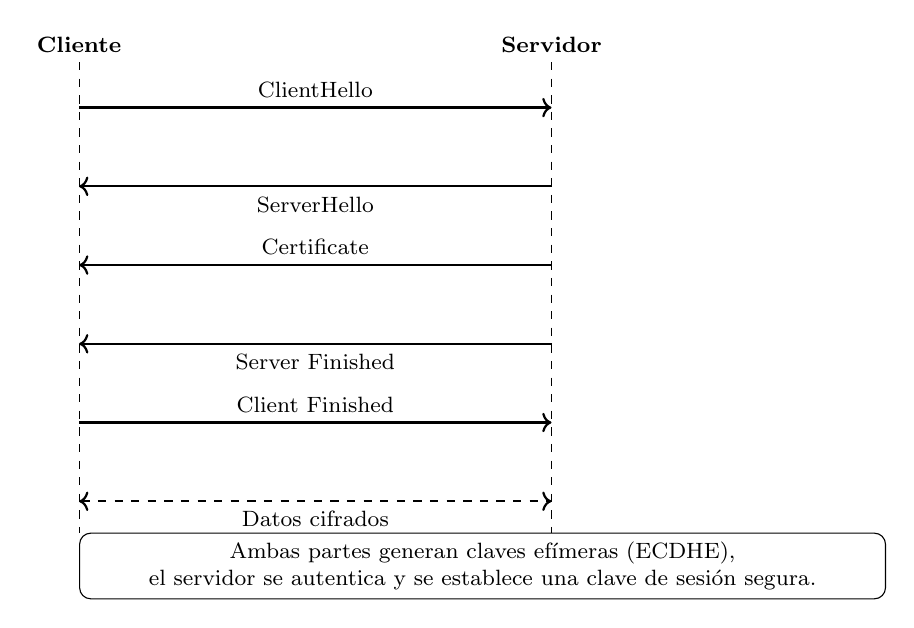
\begin{tikzpicture}[font=\footnotesize, node distance=1.2cm]
% Columnas Cliente y Servidor
\node (client) at (0,0) {\textbf{Cliente}};
\node (server) at (6,0) {\textbf{Servidor}};

% Líneas verticales
\draw[dashed] (client) -- +(0,-6.2);
\draw[dashed] (server) -- +(0,-6.2);

% Flujo de mensajes (con espacio más amplio)
\draw[->, thick] (0,-0.8) -- (6,-0.8) node[midway, above] {ClientHello};
\draw[<-, thick] (0,-1.8) -- (6,-1.8) node[midway, below] {ServerHello};
\draw[<-, thick] (0,-2.8) -- (6,-2.8) node[midway, above] {Certificate};
\draw[<-, thick] (0,-3.8) -- (6,-3.8) node[midway, below] {Server Finished};
\draw[->, thick] (0,-4.8) -- (6,-4.8) node[midway, above] {Client Finished};
\draw[<->, thick, dashed] (0,-5.8) -- (6,-5.8) node[midway, below] {Datos cifrados};

% Etiqueta inferior
\node[draw, rounded corners, text width=10cm, align=center, below=6.4cm of client, anchor=west]
{Ambas partes generan claves efímeras (ECDHE),\\ el servidor se autentica y se establece una clave de sesión segura.};

\end{tikzpicture}
\caption{Handshake simplificado del protocolo TLS 1.3.}
\end{figure}


\subsection{Primitivas Criptográficas Utilizadas}

TLS 1.3 emplea primitivas modernas y seguras, eliminando mecanismos obsoletos.  
Entre las principales se encuentran:

\begin{itemize}
    \item \textbf{Cifrado simétrico:} AES-GCM y ChaCha20-Poly1305 para proporcionar confidencialidad e integridad.
    \item \textbf{Intercambio de claves:} ECDHE (Elliptic Curve Diffie-Hellman Ephemeral), garantizando secreto perfecto hacia adelante.
    \item \textbf{Firmas digitales:} Ed25519, ECDSA o RSA-PSS, utilizadas para autenticar entidades.
    \item \textbf{Funciones hash:} SHA-256 y SHA-384, usadas en el cálculo de claves y autenticación.
\end{itemize}

\subsection{Cumplimiento de los Objetivos de Seguridad}

\subsubsection*{Confidencialidad}
Los datos se cifran con una clave simétrica derivada del intercambio ECDHE, impidiendo que terceros interpreten la información incluso si interceptan el tráfico.

\[
C = E_{K_{sym}}(M)
\]

\subsubsection*{Integridad}
TLS 1.3 emplea modos AEAD (Authenticated Encryption with Associated Data), que proporcionan cifrado y verificación de integridad en una sola operación.

\[
Tag = MAC(K_{auth}, M)
\]

\subsubsection*{Autenticación}
Durante el \textit{Handshake}, el servidor presenta su certificado digital y prueba su autenticidad firmando datos con su clave privada.  
El cliente puede opcionalmente autenticarse de la misma forma.

\subsection{Aplicaciones Modernas de TLS}

TLS 1.3 es hoy un pilar fundamental en la seguridad de Internet y sistemas corporativos.  
Algunos ejemplos concretos incluyen:

\begin{itemize}
    \item \textbf{HTTPS (Navegación Web Segura):} Sitios como Google, Amazon o Wikipedia usan TLS 1.3 para cifrar las conexiones, evitando espionaje o manipulación de datos.
    \item \textbf{Correo Electrónico Seguro:} Servidores como Gmail y Outlook emplean SMTPS, POP3S e IMAPS para proteger credenciales y contenido de mensajes.
    \item \textbf{Servicios en la Nube:} Plataformas como AWS, Azure o Google Cloud aseguran sus APIs y paneles administrativos con TLS 1.3.
    \item \textbf{Aplicaciones de Mensajería y Videollamadas:} WhatsApp Web, Zoom y Microsoft Teams cifran sus canales de control y autenticación mediante TLS.
    \item \textbf{VPNs Empresariales:} Soluciones como OpenVPN o WireGuard utilizan TLS o sus derivados para establecer túneles cifrados entre sedes o empleados remotos.
\end{itemize}

En conjunto, TLS 1.3 no solo protege la confidencialidad, sino también la confianza en la infraestructura digital moderna.

\newpage
\section*{Pregunta 4: Diseño de un Sistema con No Repudio Verificable}

\subsection{Sistema de Firma Electrónica Segura}

En el enunciado se planeta el siguiente escenario:

\begin{quote}

Se requiere diseñar una arquitectura para un sistema de \textbf{firma electrónica de contratos}, denominado \textbf{SECS (Secure Electronic Contract Signing System)}, en el cual dos partes: \textbf{Alice} (proveedora del servicio) y \textbf{Bob} (cliente), deben firmar digitalmente un contrato electrónico con plena validez jurídica.

El sistema debe garantizar:
\begin{itemize}
    \item \textbf{No Repudio de Origen:} Ninguna de las partes puede negar haber firmado el contrato.
    \item \textbf{No Repudio de Recepción:} Ninguna de las partes puede negar haber recibido el documento firmado.
\end{itemize}

Ambas propiedades son esenciales para asegurar la \textbf{validez legal, autenticidad y trazabilidad} del proceso de firma electrónica.

\end{quote}

\subsection{Requisitos Criptográficos Fundamentales}

Este sistema basa su lógica y funcionamiento en los siguientes mecanismos criptográficos:
\begin{itemize}
    \item \textbf{Infraestructura de Clave Pública:} Cada usuario tiene un par de claves $(PK, SK)$ certificado por una Autoridad.
    \item \textbf{Firmas Digitales:} Se emplea un algoritmo robusto como \textbf{RSA-PSS}.
    \item \textbf{Hash Seguro:} Se utiliza \textbf{SHA-256} para generar resúmenes únicos del contrato.
    \item \textbf{Sello de Tiempo:} Emitido por una Autoridad para asociar la firma con un instante verificable.
    \item \textbf{Registros Inmutables:} Almacenamiento en una base de datosque preserve el historial de firmas y recepciones.
\end{itemize}

\subsection{Arquitectura Propuesta del SECS}

El sistema SECS está compuesto por los siguientes módulos:

\begin{enumerate}
    \item \textbf{Módulo de Autenticación:} Verifica la identidad de los participantes mediante certificados digitales.
    \item \textbf{Módulo de Firma:} Genera y aplica la firma digital de cada parte sobre el hash del contrato.
    \item \textbf{Módulo de Notificación:} Registra y certifica la entrega del documento a la contraparte.
    \item \textbf{Autoridad de Registro:} Almacena los registros de transacciones firmadas.
    \item \textbf{Autoridad de Tiempo:} Garantiza la validez temporal de las firmas.
\end{enumerate}
\vspace{0.4cm}
\begin{figure}[h!]
\centering
\begin{tikzpicture}[
    node distance=2.2cm and 3.5cm,
    >=Latex,
    actor/.style={ellipse, draw, align=center, minimum width=2.8cm, minimum height=1.1cm, fill=gray!10},
    module/.style={rectangle, draw, rounded corners, align=center, minimum width=4cm, minimum height=1.1cm, fill=blue!5},
    storage/.style={cylinder, shape border rotate=90, draw, aspect=0.35, minimum height=1.2cm, minimum width=1cm, fill=green!5, align=center}
]

% Actores principales
\node[actor] (alice) {Alice};
\node[actor, right=7cm of alice] (bob) {Bob};

% Servidor SECS
\node[module, below=1.8cm of $(alice)!0.5!(bob)$] (secs) {Servidor SECS};

% Autoridades
\node[module, below left=2cm and 0.3cm of secs] (ca) {CA / RA};
\node[module, below right=2cm and 0.3cm of secs] (tsa) {TSA};
\node[storage, below=4.0cm of secs] (ledger) {Registro};

% ------- Flechas de comunicación principales -------
\draw[->, thick] (alice) -- node[above, sloped]{1. Envío contrato} (secs);
\draw[->, thick] (bob) -- node[above, sloped]{2. Firma} (secs);
\draw[<->, thick, dashed] (alice) -- node[below, sloped]{Contrato firmado} (bob);

% ------- Interacciones SECS con autoridades -------
\draw[->, thick] (secs) -- node[left]{Validación} (ca);
\draw[->, thick] (secs) -- node[right]{Timestamp} (tsa);
\draw[->, thick] (secs) -- node[right]{Registro} (ledger);

\end{tikzpicture}
\caption{Arquitectura simplificada del sistema SECS para firma electrónica con no repudio.}
\end{figure}


\subsection{Flujo del Protocolo SECS}

\begin{enumerate}
    \item \textbf{Inicialización:} Alice prepara el contrato \( M \) y lo envía al servidor SECS para iniciar el proceso.
    \item \textbf{Firma de Alice:} 
    \[
    Sig_A = E_{SK_A}(H(M))
    \]
    El servidor SECS solicita un sello temporal a la TSA y almacena el par \((M, Sig_A, T_A)\).
    \item \textbf{Entrega a Bob:} El contrato firmado por Alice se envía a Bob, quedando registrada la entrega.
    \item \textbf{Firma de Bob:} Bob verifica la firma de Alice, añade la suya,
    \[
    Sig_B = E_{SK_B}(H(M))
    \]
    y envía de vuelta \((M, Sig_A, Sig_B)\) al servidor.
    \item \textbf{Confirmación Final:} El servidor SECS aplica un segundo sello temporal \(T_B\) y guarda todas las evidencias en el registro inmutable.
\end{enumerate}

\subsection{Cumplimiento del No Repudio}

\begin{itemize}
    \item \textbf{No Repudio de Origen:} La firma de Alice, validada con su clave pública certificada, constituye prueba verificable del origen del documento.
    \item \textbf{No Repudio de Recepción:} La firma de Bob, junto al sello temporal y los registros del SECS, prueban que el documento fue recibido y aceptado.
\end{itemize}

Ambas pruebas pueden verificarse de forma independiente por un tercero (una autoridad legal, por ejemplo), sin intervención de los firmantes.

\subsection{Consideraciones Legales y de Seguridad}

El sistema SECS cumple con principios de las normativas internacionales como:
\begin{itemize}
    \item \textbf{Integridad de los registros:} El uso de sellos de tiempo y almacenamiento inmutable garantiza la trazabilidad y validez de las pruebas.
    \item \textbf{Auditoría:} Cualquier intento de manipular registros firmados o sellados invalidará la verificación criptográfica.
\end{itemize}

La arquitectura SECS combina mecanismos criptográficos con un diseño de protocolo robusto para lograr:
\begin{itemize}
    \item Autenticación verificable de cada firmante.
    \item Integridad total del contrato firmado.
    \item Evidencia legal inmutable de envío y recepción.
\end{itemize}

De esta forma, se ofrece una solución \textbf{técnica y jurídicamente sólida} para la firma electrónica de contratos críticos, garantizando no repudio, transparencia y validez legal.

\newpage

\section*{Bibliografía}

\begin{itemize}

    \item Chirag Bhalodia. \textit{Digital Signature Algorithm (DSA) in Network Security}. Disponible en: \url{https://www.youtube.com/watch?v=eiNZi-G-CE4}
    \item Cloudflare. \textit{Why Use TLS 1.3?}. Disponible en: \url{https://www.cloudflare.com/es-es/learning/ssl/why-use-tls-1.3/}
    \item Stallings, W. \textit{Cryptography and Network Security}, 5th Edition. Prentice Hall.

\end{itemize}


\end{document}
